% =====================================================================
% Optimization Models for Targeted Offers in Direct Marketing:
% implementation and computational study
% Paper: Talla Nobibon, Leus, Spieksma (2011), EJOR 210, 670-683
%
% Compile: xelatex main.tex (run twice; uses Source Sans 3 if installed)
% Logo: place logo-tecnico.jpg in this folder.
% Figures: python presentation/scripts/make_figures.py (from the repository root)
%
% Convention used throughout the slides:
%   * slate/grey text, blocks and tables      = content taken from the paper [1];
%   * Tecnico Blue boxes and slides with a blue badge, blue left band and blue
%     tint = the presenter's implementation, experiments and interpretation.
% =====================================================================
\documentclass[10pt,aspectratio=169]{beamer}

\usepackage{iftex}
\ifPDFTeX
  \usepackage[utf8]{inputenc}
  \usepackage[T1]{fontenc}
  \IfFileExists{sourcesanspro.sty}{\usepackage[default]{sourcesanspro}}{\IfFileExists{lmodern.sty}{\usepackage{lmodern}}{}}
\else
  \usepackage{fontspec}
  \IfFontExistsTF{Source Sans 3}{\setsansfont{Source Sans 3}}{%
    \IfFontExistsTF{Source Sans Pro}{\setsansfont{Source Sans Pro}}{}}
\fi
\usefonttheme{professionalfonts}
\usepackage{amsmath,amssymb}
\usepackage{booktabs}
\usepackage{array}
\usepackage{multirow}
\usepackage{graphicx}
\usepackage{tikz}
\usetikzlibrary{arrows.meta,positioning,calc}
\graphicspath{{figures/}}

% ---------- official colours ----------
\definecolor{tecnicoblue}{HTML}{009DE0}
\definecolor{slate}{HTML}{46555F}
\definecolor{lightgrey}{HTML}{D2D3D4}
\colorlet{bluetext}{tecnicoblue!75!black}

% ---------- classic Beamer theme (Madrid) with Tecnico colours ----------
\usetheme{Madrid}
\useinnertheme{rounded}
\useoutertheme{infolines}
\setbeamercolor{structure}{fg=tecnicoblue}
\setbeamercolor{normal text}{fg=slate!90!black,bg=white}
\setbeamercolor{palette primary}{bg=tecnicoblue,fg=white}
\setbeamercolor{palette secondary}{bg=slate,fg=white}
\setbeamercolor{palette tertiary}{bg=slate!85!black,fg=white}
\setbeamercolor{palette quaternary}{bg=slate!85!black,fg=white}
\setbeamercolor{frametitle}{bg=white,fg=slate!95!black}
\setbeamercolor{title rule}{bg=tecnicoblue}
\setbeamercolor{title}{bg=tecnicoblue,fg=white}
\setbeamercolor{subtitle}{fg=white}
\setbeamercolor{alerted text}{fg=slate!95!black}
\setbeamercolor{block title}{bg=slate,fg=white}
\setbeamercolor{block body}{bg=lightgrey!30,fg=slate!90!black}
\setbeamercolor{item projected}{bg=slate,fg=white}
\setbeamercolor{item}{fg=slate}
\setbeamercolor{subitem}{fg=slate!80}
\setbeamercolor{section number projected}{bg=slate,fg=white}
\setbeamercolor{section in toc}{fg=slate!90!black}
\setbeamerfont{frametitle}{series=\bfseries}
\setbeamerfont{title}{series=\bfseries}
\setbeamerfont{author}{size=\normalsize}
\setbeamerfont{institute}{size=\scriptsize}
\setbeamerfont{date}{size=\footnotesize}
\setbeamerfont{block title}{series=\bfseries}
\setbeamertemplate{navigation symbols}{}
\setbeamertemplate{frametitle continuation}{}
\setbeamerfont{footnote}{size=\scriptsize}
\setbeamercolor{footnote}{fg=slate}
\setbeamercolor{footnote mark}{fg=slate}
\setbeamertemplate{bibliography item}{[\theenumiv]}
\setbeamercolor{bibliography entry author}{fg=slate!90!black}
\setbeamercolor{bibliography entry title}{fg=slate!90!black}
\setbeamercolor{bibliography entry location}{fg=slate!70}
\setbeamercolor{bibliography entry note}{fg=slate!70}
\setbeamertemplate{blocks}[rounded][shadow=true]
\setbeamertemplate{itemize items}[circle]
\setbeamertemplate{enumerate items}[circle]
\setbeamertemplate{sections/subsections in toc}[circle]

% ---------- frame title: white bar, title, logo, blue rule ----------
\newcommand{\tecnicologo}[1]{\IfFileExists{logo-tecnico.jpg}{\includegraphics[height=#1]{logo-tecnico.jpg}}{}}
\setbeamertemplate{frametitle}{%
  \nointerlineskip
  \begin{beamercolorbox}[wd=\paperwidth,ht=0.80cm,dp=0.25cm,leftskip=0.35cm,rightskip=0.35cm]{frametitle}%
    \usebeamerfont{frametitle}\insertframetitle\hfill
    \raisebox{-0.10cm}{\tecnicologo{0.58cm}}%
  \end{beamercolorbox}%
  \par\nointerlineskip
  \begin{beamercolorbox}[wd=\paperwidth,ht=1.5pt,dp=0pt]{title rule}\end{beamercolorbox}%
  \par\vspace{2pt}}

% ---------- presenter's material: always in Tecnico Blue ----------
\setbeamercolor{own title}{bg=tecnicoblue,fg=white}
\setbeamercolor{own body}{bg=tecnicoblue!7,fg=slate!95!black}
\newenvironment{ownbox}[2]{%
  \begin{beamerboxesrounded}[upper=own title,lower=own body,shadow=false]%
    {\small\bfseries #1\if\relax\detokenize{#2}\relax\else{\normalfont\itshape\ (#2)}\fi}\small}%
  {\end{beamerboxesrounded}}
\newenvironment{remarkbox}[1][]{\begin{ownbox}{Remark}{#1}}{\end{ownbox}}
\newenvironment{findingbox}[1][]{\begin{ownbox}{Finding}{#1}}{\end{ownbox}}
\newcommand{\ownbadge}[1]{#1: }
\newcommand{\ownband}{\nointerlineskip\vbox to 0pt{%
  \begin{tikzpicture}[remember picture,overlay]
    \fill[tecnicoblue] ([yshift=-1.12cm]current page.north west) rectangle ([xshift=0.18cm,yshift=0.42cm]current page.south west);
  \end{tikzpicture}\vss}}
\newenvironment{ownslide}{\setbeamercolor{background canvas}{bg=tecnicoblue!4}}{}

\newcounter{figno}
\newcommand{\figcap}[1]{\refstepcounter{figno}{\scriptsize\textbf{Figure~\thefigno.} #1\par}}
% ---------- notation helpers ----------
\newcommand{\ok}{\textcolor{slate}{\checkmark}}
\newcommand{\dev}{\textcolor{bluetext}{\bfseries deviation}}

\title[Targeted offers in direct marketing]{Optimization Models for Targeted Offers in Direct Marketing}
\subtitle{Implementation and computational study of the exact formulations\\[3pt]
\small after F.~Talla Nobibon, R.~Leus, F.C.R.~Spieksma, \emph{EJOR} 210 (2011) 670--683}
\author[J.~Cavalcante (ist431224)]{Judecir Cavalcante\\ {\small ist431224}}
\institute[DEG, IST]{PhD Programme in Engineering and Management\\
Department of Engineering and Management\\
Instituto Superior T\'ecnico, Universidade de Lisboa}
\date[Homework 3]{Optimization and Applications\\
Prof.~Jos\'e Rui Figueira\\
Homework 3}

\begin{document}

% =====================================================================
% Cover and outline (not counted)
% =====================================================================
\begin{frame}[plain,noframenumbering]
  \IfFileExists{logo-tecnico.jpg}{\begin{center}\tecnicologo{1.1cm}\end{center}\vspace{-6pt}}{}
  \vspace{-6pt}
  \titlepage
  \vspace{-10pt}
  \begin{center}
    \scriptsize\itshape Problem and models follow \cite{tallanobibon2011}.
    {\color{tecnicoblue}\upshape\bfseries Blue} marks the presenter's implementation, experiments and interpretation.
  \end{center}
\end{frame}

\begin{frame}[noframenumbering]{Outline}
  \tableofcontents
\end{frame}

% =====================================================================
\section{Problem and data}
% =====================================================================

% ---- 1 ----
\begin{frame}{The problem}
  \vspace{-4pt}
  \small
  \begin{itemize}
    \item A \textbf{direct-marketing campaign} offers products to selected customers. The paper addresses
          \emph{retention} campaigns, which seek additional revenue from existing customers of a bank
          \cite{tallanobibon2011}.
    \item Response models estimate the expected return $p_{ij}=r_{ij}\,DFV_{ij}$ of offering product $j$ to customer $i$
          (acceptance probability times value to the firm); these estimates are \textbf{inputs} of the model.
  \end{itemize}
  \begin{block}{Product targeting problem}
    \small Decide which products to offer to which customers so as to maximize the expected net profit of the campaign,
    subject to four business requirements:
    \begin{enumerate}
      \item a corporate \textbf{hurdle rate} $R$ on the return on investment;
      \item a \textbf{budget} $B_j$ per product, because each business unit funds its own product;
      \item a maximum number $M_i$ of \textbf{offers per customer};
      \item a \textbf{minimum-quantity commitment} (MQC) $O_j$: a product used in the campaign is offered to at least $O_j$ customers.
    \end{enumerate}
    A \textbf{fixed cost} $f_j$ is incurred whenever product $j$ is used.
  \end{block}
  \vspace{-4pt}\footnotesize The problem is strongly NP-hard; even finding a solution with positive profit is NP-hard \cite{tallanobibon2011}.
\end{frame}

% ---- 2 ----
\begin{ownslide}
\begin{frame}{\ownbadge{Implementation}Instance generation}
  \ownband
  \small
  Instances follow the rules of Section~5.1 of \cite{tallanobibon2011}, with $C_j=\sum_i c_{ij}$ and $\bar M=\sum_i M_i/n$.

  \vspace{4pt}
  \centering\footnotesize
  \renewcommand{\arraystretch}{1.15}
  \begin{tabular}{@{}lll@{}}
    \toprule
    \textbf{Parameter} & \textbf{Meaning} & \textbf{Rule}\\
    \midrule
    $c_{ij}$, $p_{ij}$ & cost and expected return of an offer & integers in $\{1,2,3\}$ and $\{0,\dots,16\}$\\
    $R$ & hurdle rate & $5\%$, $10\%$ or $15\%$\\
    $M_i$, variant s & few offers per customer & between $1$ and $n/5$\\
    $M_i$, variant $\ell$ & many offers per customer & between $\lceil n/3\rceil$ and $\lceil 2n/3\rceil$\\
    $O_j$ & minimum-quantity commitment & between $\bar M$ and $2\bar M$\\
    $B_j$ & budget: minimum, maximum or random & between $O_jC_j/m$ and $2\bar M C_j/m$\\
    $f_j$ & fixed cost & proportional to $O_j$ and to the margin of product $j$\\
    \bottomrule
  \end{tabular}

  \vspace{8pt}
  \raggedright
  \begin{ownbox}{Implementation}{}
    \begin{itemize}
      \item The generator follows these rules, with two small adjustments (rounding of $O_j$ and range of the random budget) that keep the budgets consistent.
      \item Instances are reproducible from a fixed seed. Because the seed is the same, instances with the same $n$ share their costs and returns.
    \end{itemize}
  \end{ownbox}
\end{frame}
\end{ownslide}

% =====================================================================
\section{Formulations}
% =====================================================================

% ---- 3 ----
\begin{frame}{Model M1}
  \vspace{-4pt}
  \small
  Variables: $x_{ij}=1$ if product $j$ is offered to customer $i$; $y_j=1$ if product $j$ is used in the campaign.
  {\setlength{\abovedisplayskip}{2pt}\setlength{\belowdisplayskip}{2pt}\setlength{\jot}{1pt}
  \begin{align*}
    \max\ & \sum\nolimits_{i,j}(p_{ij}-c_{ij})\,x_{ij}-\sum\nolimits_{j}f_j\,y_j && (1)\ \text{net profit}\\
    \text{s.t.}\ & \sum\nolimits_{i,j}p_{ij}x_{ij}\ \ge\ (1+R)\Big[\sum\nolimits_{i,j}c_{ij}x_{ij}+\sum\nolimits_{j}f_j y_j\Big] && (2)\ \text{hurdle rate}\\
    & \sum\nolimits_{i}c_{ij}x_{ij}\le B_j, && j=1,\dots,n \quad (3)\ \text{budget}\\
    & \sum\nolimits_{j}x_{ij}\le M_i, && i=1,\dots,m \quad (4)\ \text{offers per customer}\\
    & \sum\nolimits_{i}x_{ij}\le m\,y_j, && j=1,\dots,n \quad (5)\ \text{linking}\\
    & \sum\nolimits_{i}x_{ij}\ge O_j\,y_j, && j=1,\dots,n \quad (6)\ \text{MQC}\\
    & x_{ij},\,y_j\in\{0,1\}. && (7)
  \end{align*}}
  \vspace{-4pt}
  \footnotesize
  \begin{itemize}
    \item (M1) has $mn+n$ binary variables and $1+m+3n$ constraints. Constraints (5) and (6) together state that
          a product is either unused or offered to at least $O_j$ customers.
    \item In the LP relaxation, (5) $\sum_i x_{ij}\le m\,y_j$ allows $y_j=\sum_i x_{ij}/m$, so the fixed cost $f_j$ is charged
          at a rate of only $f_j/m$ per offer. This weakens the LP bound of (M1).
  \end{itemize}
\end{frame}

% ---- 4 ----
\begin{frame}{Model M2}
  \small
  (M2) replaces the aggregated linking constraints (5) $\sum_i x_{ij}\le m\,y_j$ by their \textbf{disaggregated} form
  \[
    x_{ij}\le y_j,\qquad i=1,\dots,m,\ j=1,\dots,n. \qquad (8)
  \]
  \begin{block}{Proposition 3 \cite{tallanobibon2011}}
    The convex hull of the feasible solutions of (M1) equals the convex hull of the solutions satisfying
    (2)--(4), (6) and (8), with $0\le y_j\le 1$ and $x_{ij}\in\{0,1\}$.
  \end{block}
  \begin{itemize}
    \item Summing (8) over $i$ gives (5); hence every LP solution of (M2) is an LP solution of (M1), and
          $z^{LP}_{(M2)}\le z^{LP}_{(M1)}$.
    \item In the paper, (M2) also relaxes $y_j\in\{0,1\}$ to $0\le y_j\le 1$. It has $mn-n$ more constraints than (M1): $mn$ constraints (8) replace the $n$ constraints (5).
    \item In the paper, (M2) is the formulation solved with CPLEX 10.2.
  \end{itemize}
  \begin{remarkbox}[implementation]
    The implementation keeps $y_j\in\{0,1\}$ in the integer version of (M2). By Proposition 3 this does not change the optimal value,
    and the LP relaxation is the same, since $x$ and $y$ are relaxed to $[0,1]$ in both cases.
  \end{remarkbox}
\end{frame}

% ---- 5 ----
\begin{frame}{Model M3}
  \vspace{-6pt}
  \small
  For each product $j$, let $S_{pj}$, $p=1,\dots,k_j$, be the sets of customers with $|S_{pj}|\ge O_j$ and
  $\sum_{i\in S_{pj}}c_{ij}\le B_j$. The binary variable $z_{pj}$ equals $1$ if product $j$ is offered exactly to $S_{pj}$.
  {\setlength{\abovedisplayskip}{2pt}\setlength{\belowdisplayskip}{2pt}\setlength{\jot}{1pt}
  \begin{align*}
    \max\ & \sum\nolimits_{j}\sum\nolimits_{p}\Big[\sum\nolimits_{i\in S_{pj}}(p_{ij}-c_{ij})-f_j\Big]z_{pj} && (9)\\
    \text{s.t.}\ & \sum\nolimits_{j}\sum\nolimits_{p}\Big[\sum\nolimits_{i\in S_{pj}}\big(p_{ij}-(1+R)c_{ij}\big)-(1+R)f_j\Big]z_{pj}\ge 0 && (10)\ \text{hurdle rate}\\
    & \sum\nolimits_{j}\sum\nolimits_{p:\,i\in S_{pj}}z_{pj}\le M_i, \qquad i=1,\dots,m && (11)\ \text{offers per customer}\\
    & \sum\nolimits_{p=1}^{k_j}z_{pj}\le 1, \qquad j=1,\dots,n && (12)\ \text{one set per product}\\
    & z_{pj}\in\{0,1\}. && (13)
  \end{align*}}
  \vspace{-6pt}
  \footnotesize
  \begin{itemize}
    \item Budget (3) and MQC (6) are built into the definition of the columns. (M3) results from a Dantzig--Wolfe decomposition,
          and $z^{\star}\le z^{LP}_{(M3)}\le z^{LP}_{(M2)}$ \cite{tallanobibon2011}.
    \item The number of columns grows as $O(n\,2^m)$. The paper solves (M3) by column generation within branch-and-price.
  \end{itemize}
  \begin{remarkbox}[implementation]
    The implementation enumerates all admissible columns explicitly and is therefore restricted to $m\le 12$.
    Branch-and-price is not implemented. The solution of (M3) is mapped back to $(x,y)$ and checked against (2)--(7).
  \end{remarkbox}
\end{frame}

% =====================================================================
\section{Implementation}
% =====================================================================

% ---- implementation overview ----
\begin{ownslide}
\begin{frame}{\ownbadge{Implementation}Overview}
  \ownband
  \centering
  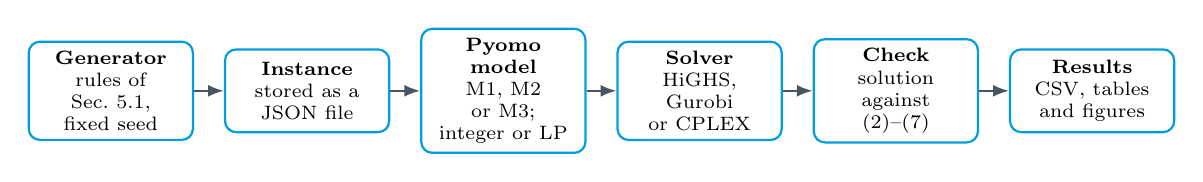
\begin{tikzpicture}[font=\scriptsize,
      box/.style={draw=tecnicoblue,thick,rounded corners,fill=white,align=center,text width=1.85cm,minimum height=1.05cm},
      arr/.style={-{Latex[length=2mm]},thick,slate}]
    \node[box] (gen) {\textbf{Generator}\\ rules of Sec.~5.1,\\ fixed seed};
    \node[box,right=0.38cm of gen] (inst) {\textbf{Instance}\\ stored as a\\ JSON file};
    \node[box,right=0.38cm of inst] (mod) {\textbf{Pyomo model}\\ M1, M2 or M3;\\ integer or LP};
    \node[box,right=0.38cm of mod] (sol) {\textbf{Solver}\\ HiGHS, Gurobi\\ or CPLEX};
    \node[box,right=0.38cm of sol] (chk) {\textbf{Check}\\ solution against\\ (2)--(7)};
    \node[box,right=0.38cm of chk] (res) {\textbf{Results}\\ CSV, tables\\ and figures};
    \foreach \a/\b in {gen/inst,inst/mod,mod/sol,sol/chk,chk/res} \draw[arr] (\a) -- (\b);
  \end{tikzpicture}

  \vspace{10pt}
  \raggedright
  \begin{itemize}
    \item \textbf{Pyomo as a common modelling layer.} Each formulation is written once, in algebraic form close to the paper,
          and sent to HiGHS, Gurobi or CPLEX by changing only the solver name.
    \item \textbf{M1 and M2 share one model builder}; they differ only in the linking constraints, (5) or (8).
          The LP relaxation changes the domain of the variables from $\{0,1\}$ to $[0,1]$.
    \item \textbf{M3 in two steps:} all admissible columns are enumerated, then the set-covering model is built from them.
    \item \textbf{Every solution is checked} against (2)--(7) by an independent function, and unit tests cover a small example solved by brute force.
  \end{itemize}
\end{frame}
\end{ownslide}

% =====================================================================
\section{Experimental design}
% =====================================================================

% ---- 6 ----
\begin{ownslide}
\begin{frame}{\ownbadge{Design}Experiments}
  \ownband
  \small
  \begin{columns}[T]
    \begin{column}{0.48\textwidth}
      \begin{ownbox}{Experiment 1}{small instances}
        \begin{itemize}
          \item 50 instances with $m=4,\dots,12$ customers and $n=2,\dots,5$ products.
          \item Models \textbf{M1, M2 and M3}.
          \item Goal: validate the three models and compare their LP bounds.
        \end{itemize}
      \end{ownbox}
    \end{column}
    \begin{column}{0.48\textwidth}
      \begin{ownbox}{Experiment 2}{groups S1, S2, S3 of the paper}
        \begin{itemize}
          \item 162 instances with $m=100$, 200, 300 customers and $n=5$, 10, 15 products.
          \item Models \textbf{M1 and M2} (M3 needs column generation at this size).
          \item Goal: compare bounds and solve times as $m$ grows.
        \end{itemize}
      \end{ownbox}
    \end{column}
  \end{columns}
  \vspace{6pt}
  In both experiments, each instance is solved as an integer program and as an LP relaxation, with \textbf{HiGHS, Gurobi and CPLEX}.
  \vspace{6pt}
  \begin{ownbox}{Computational environment}{}
    \footnotesize
    \renewcommand{\arraystretch}{1.1}
    \begin{tabular}{@{}ll@{}}
      Machine & Intel Core i7-8565U @ 1.80\,GHz (4 cores, 8 threads), 15.8\,GB RAM, Windows~10\\
      Software & Python 3.12.10, Pyomo 6.10.1\\
      Solvers & HiGHS 1.15.1, Gurobi 13.0.3, CPLEX 22.2.0.0, with default settings\\
      Time limit & 300\,s (Experiment 1) and 3600\,s (Experiment 2) per run\\
    \end{tabular}
  \end{ownbox}
\end{frame}
\end{ownslide}

% =====================================================================
\section{Experiment 1: small instances}
% =====================================================================

% ---- 7 ----
\begin{ownslide}
\begin{frame}{\ownbadge{Experiment 1}LP bounds}
  \ownband
  \small
  \begin{itemize}
    \item The three models and the three solvers return the same optimum $z^{\star}$ on all 50 instances.
    \item The LP gap $100\,(z^{LP}-z^{\star})/z^{\star}$ depends only on the model, and
          $z^{\star}\le z^{LP}_{(M3)}\le z^{LP}_{(M2)}\le z^{LP}_{(M1)}$ holds in every instance.
  \end{itemize}
  \begin{columns}[c]
    \begin{column}{0.55\textwidth}
      \centering
      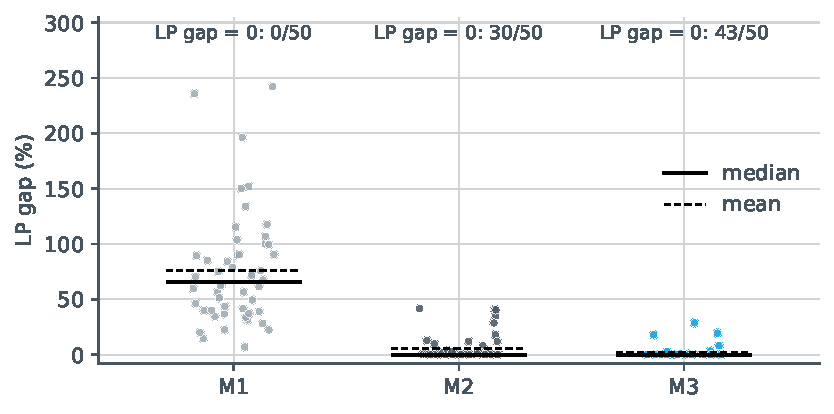
\includegraphics[width=\linewidth]{exp1_lp_gap.pdf}\\[-2pt]
      \raggedright\figcap{LP gap of M1, M2 and M3 on the 50 instances of Experiment 1; one point per instance.}
    \end{column}
    \begin{column}{0.43\textwidth}
      \centering\footnotesize
      \begin{tabular}{@{}lrrrr@{}}
        \toprule
        & \multicolumn{3}{c}{LP gap (\%)} & LP gap\\
        \cmidrule(lr){2-4}
        Model & mean & median & max & $=0$\\
        \midrule
        M1 & 75.90 & 65.63 & 242.22 & 0/50\\
        M2 & 5.63 & 0.00 & 41.67 & 30/50\\
        M3 & 1.63 & 0.00 & 28.75 & 43/50\\
        \bottomrule
      \end{tabular}\\[8pt]
      \raggedright\small
      The LP relaxation of M3 already gives the integer optimum in 43 of 50 instances.
    \end{column}
  \end{columns}
\end{frame}
\end{ownslide}

% ---- 8 ----
\begin{ownslide}
\begin{frame}{\ownbadge{Experiment 1}Size of M3}
  \ownband
  \vspace{-2pt}
  \centering
  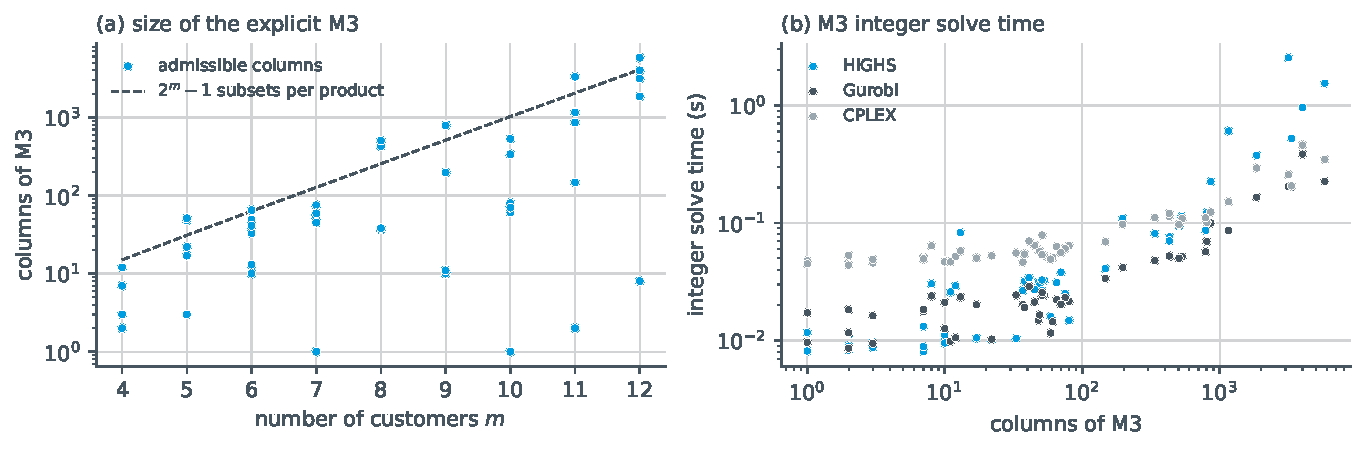
\includegraphics[width=0.88\textwidth]{exp1_columns_time.pdf}\\[-2pt]
  \figcap{(a) Admissible columns of M3 per instance, as a function of $m$. (b) Integer solve time of M3 against its number of columns, per solver. Logarithmic scales.}

  \vspace{4pt}
  \raggedright
  \begin{itemize}
    \item The number of columns ranges from 1 to 5\,809, already with at most 12 customers.
    \item The solve time of M3 increases with the number of columns, but stays below 2.6\,s.
    \item M1 and M2 are solved in less than 0.2\,s on every instance; at this size the times are too small to rank the solvers.
  \end{itemize}
\end{frame}
\end{ownslide}

% ---- 9 ----
% ---- 10 ----
% =====================================================================
\section{Experiment 2: groups S1 to S3}
% =====================================================================

% ---- E2: optimality ----
% ---- E2: LP bounds ----
\begin{ownslide}
\begin{frame}{\ownbadge{Experiment 2}LP bounds}
  \ownband
  \vspace{-2pt}
  \centering
  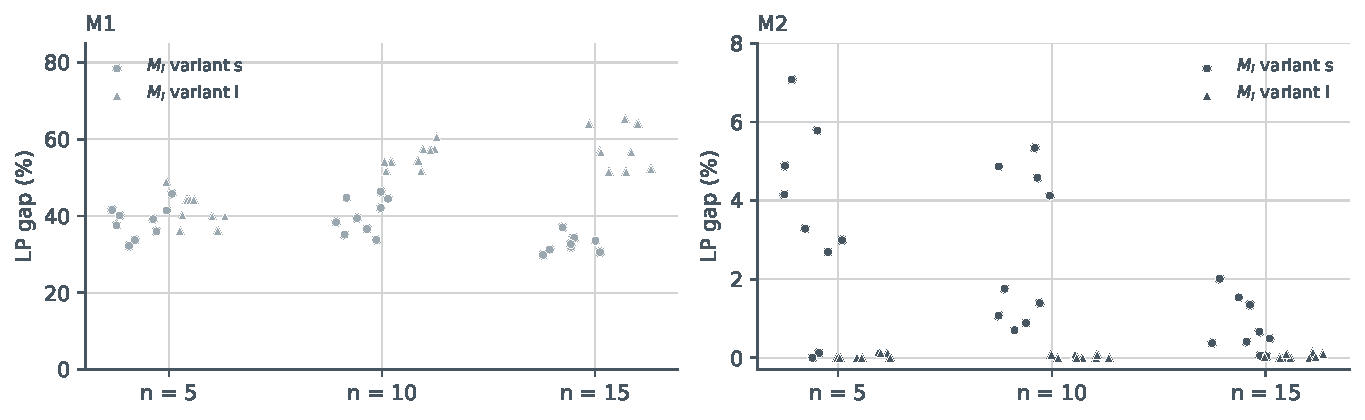
\includegraphics[width=0.70\textwidth]{exp2_lp_gap.pdf}\\[-2pt]
  \figcap{LP gap of M1 (left) and M2 (right) on the 162 instances, by group and $M_i$ variant. The vertical scales differ.}

  \vspace{3pt}
  \footnotesize
  \begin{tabular}{@{}l|rr|rr@{}}
    \toprule
    & \multicolumn{2}{c|}{M1: LP gap (\%)} & \multicolumn{2}{c}{M2: LP gap (\%)}\\
    Group & mean & max & mean & max\\
    \midrule
    S1 ($m=100$) & 44.36 & 65.30 & 1.18 & 7.08\\
    S2 ($m=200$) & 51.61 & 73.09 & 0.87 & 6.90\\
    S3 ($m=300$) & 52.24 & 78.82 & 1.76 & 11.08\\
    \bottomrule
  \end{tabular}

  \vspace{4pt}
  \raggedright\small
  \begin{itemize}
    \item All 972 integer runs end with status optimal and the models agree on the optimum; three runs on S3 stop at the
          solver tolerance ($0.01\%$), one unit away from it.
    \item The LP gap of M2 is about 1\% on average, against 44--52\% for M1, in every group.
  \end{itemize}
\end{frame}
\end{ownslide}

% ---- E2: solve times ----
\begin{ownslide}
\begin{frame}{\ownbadge{Experiment 2}Solve times}
  \ownband
  \vspace{-2pt}
  \centering
  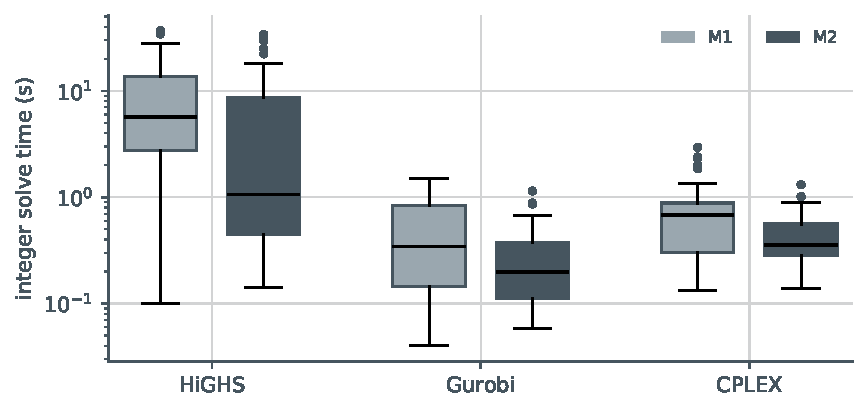
\includegraphics[width=0.64\textwidth]{exp2_time_boxplot.pdf}\\[-2pt]
  \figcap{Integer solve time of M1 and M2 per solver, for each group (54 instances per box). Logarithmic scale.}

  \vspace{3pt}
  \footnotesize
  \begin{tabular}{@{}ll|rr|rr|rr@{}}
    \toprule
    & & \multicolumn{2}{c|}{S1 ($m=100$)} & \multicolumn{2}{c|}{S2 ($m=200$)} & \multicolumn{2}{c}{S3 ($m=300$)}\\
    Solver & Model & median & max & median & max & median & max\\
    \midrule
    HiGHS  & M1 & 5.68 & 36.71 & 7.33 & 193.25 & 22.65 & 1\,128.02\\
           & M2 & 1.07 & 33.85 & 2.32 & 122.02 & 7.97 & 139.14\\
    Gurobi & M1 & 0.34 & 1.49 & 0.57 & 3.76 & 1.21 & 10.02\\
           & M2 & 0.20 & 1.14 & 0.36 & 5.06 & 0.56 & 6.50\\
    CPLEX  & M1 & 0.68 & 2.95 & 0.74 & 10.59 & 0.99 & 1\,145.38\\
           & M2 & 0.35 & 1.31 & 0.60 & 6.21 & 0.72 & 7.15\\
    \bottomrule
  \end{tabular}

  \vspace{4pt}
  \raggedright\small
  \begin{itemize}
    \item Gurobi and CPLEX solve a typical instance in about one second; HiGHS is roughly 7 to 9 times slower than Gurobi on M2.
  \end{itemize}
\end{frame}
\end{ownslide}

% ---- E2: effect of m ----
% ---- E2: M1 versus M2 ----
\begin{ownslide}
\begin{frame}{\ownbadge{Experiment 2}M1 versus M2}
  \ownband
  \vspace{-2pt}
  \centering
  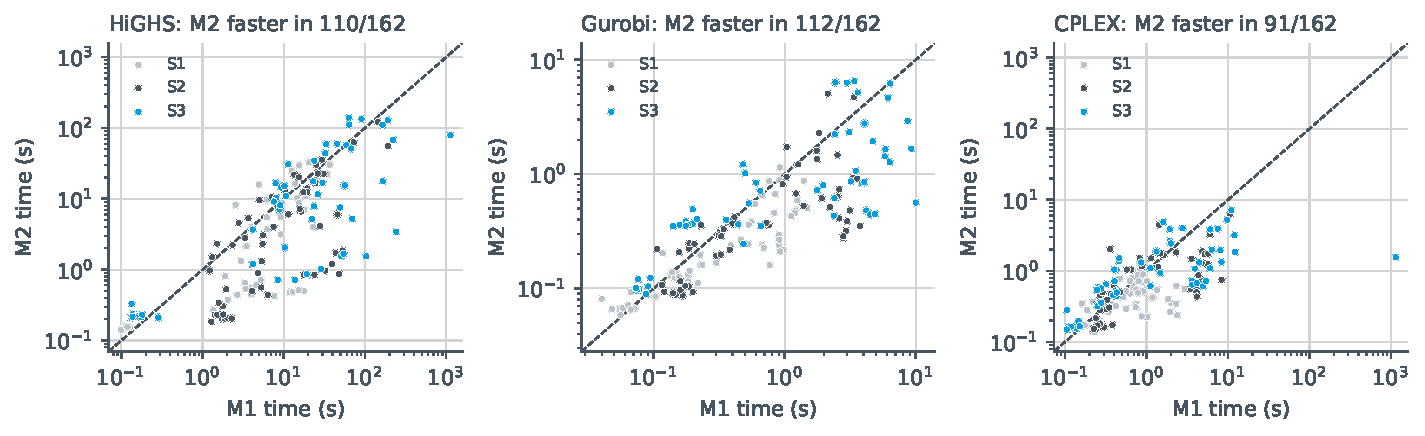
\includegraphics[width=0.63\textwidth]{exp2_paired_time.pdf}\\[-2pt]
  \figcap{Ratio between the integer solve times of M2 and M1 on the same instance, per group and solver (54 instances per box, logarithmic scale). Values below 1 mean that M2 is faster.}

  \vspace{3pt}
  \footnotesize
  \begin{tabular}{@{}l|ccc|ccc@{}}
    \toprule
    & \multicolumn{3}{c|}{instances where M2 is faster} & \multicolumn{3}{c}{geometric mean of time(M2)/time(M1)}\\
    Group & HiGHS & Gurobi & CPLEX & HiGHS & Gurobi & CPLEX\\
    \midrule
    S1 & 35/54 & 44/54 & 36/54 & 0.46 & 0.66 & 0.69\\
    S2 & 43/54 & 41/54 & 34/54 & 0.31 & 0.59 & 0.65\\
    S3 & 32/54 & 27/54 & 21/54 & 0.44 & 0.71 & 0.75\\
    \bottomrule
  \end{tabular}

  \vspace{4pt}
  \raggedright\small
  \begin{itemize}
    \item M2 is faster on average with every solver, but not on every instance.
    \item The time difference is much smaller than the difference in LP gap: the solvers probably strengthen M1 on their own
          (CPLEX solves 155 of the 162 M1 instances at the root node).
  \end{itemize}
\end{frame}
\end{ownslide}

% ---- E2: small versus large M_i ----
\begin{ownslide}
\begin{frame}{\ownbadge{Experiment 2}Small versus large $M_i$}
  \ownband
  Variant s: each customer accepts few offers. Variant $\ell$: each customer accepts many. Each variant has 81 instances.

  \vspace{8pt}
  \centering\small
  \renewcommand{\arraystretch}{1.15}
  \begin{tabular}{@{}l|rr|rrr@{}}
    \toprule
    & \multicolumn{2}{c|}{mean LP gap (\%)} & \multicolumn{3}{c}{mean time of M2 (s)}\\
    Variant & M1 & M2 & HiGHS & Gurobi & CPLEX\\
    \midrule
    s (few offers)       & 42.05 & 2.43 & 24.74 & 1.14 & 1.35\\
    $\ell$ (many offers) & 56.76 & 0.10 & 3.05  & 0.37 & 0.55\\
    \bottomrule
  \end{tabular}

  \vspace{10pt}
  \raggedright\normalsize
  \begin{itemize}
    \item \textbf{Variant s is the harder case}: larger LP gap of M2 and solve times 2.5 to 8 times longer.
    \item \textbf{In variant $\ell$, the LP relaxation of M2 is almost integral} (zero gap in 45 of 81 instances), and M2 gains most over M1.
    \item A possible explanation: when customers accept few offers, the products compete for the same customers.
  \end{itemize}
\end{frame}
\end{ownslide}

% ---- E2: conclusions ----
% =====================================================================
\section{Summary}
% =====================================================================

% ---- 16 ----
\begin{ownslide}
\begin{frame}{\ownbadge{Summary}Conclusions and limitations}
  \ownband
  \textbf{Conclusions}
  \begin{itemize}
    \item The three exact formulations of the paper were implemented and validated: all models and solvers agree on the optimum.
    \item The LP bounds follow the theory: M3 is the strongest and M1 by far the weakest. The disaggregated constraints (8) give most of the improvement.
    \item M2 is also faster on average and more robust than M1: its worst case is 139\,s, against about 1\,100\,s for M1.
    \item Up to $m=300$, M2 with a commercial solver is enough: at most 7.2\,s per instance with Gurobi or CPLEX; HiGHS is several times slower.
    \item Instances where customers accept few offers are the harder ones.
  \end{itemize}
  \vspace{8pt}
  \textbf{Limitations}
  \begin{itemize}
    \item M3 is solved only by enumeration ($m\le12$); column generation and branch-and-price are not implemented.
    \item Only the small groups (S1 to S3) were run, with one seed and one run per instance.
    \item The instances are generated by the rules of the paper, but they are not the paper's instances.
  \end{itemize}
\end{frame}
\end{ownslide}

% =====================================================================
% Thank you (not counted)
% =====================================================================
\begin{frame}[plain,noframenumbering]
  \begin{tikzpicture}[remember picture,overlay]
    \node[fill=tecnicoblue,rounded corners=6pt,minimum width=0.55\paperwidth,
          minimum height=2.6cm,align=center,text=white]
      (ty) at ([yshift=1.7cm]current page.center)
      {{\fontsize{30}{34}\selectfont\bfseries Thank you}\\[8pt]{\Large Questions?}};
    \node[below=0.35cm of ty] {\tecnicologo{0.9cm}};
    \node[anchor=south,text=slate,font=\footnotesize,align=center] at ([yshift=0.35cm]current page.south)
      {\textbf{Judecir Cavalcante} (ist431224)\\
       PhD Programme in Engineering and Management\\
       Department of Engineering and Management\\
       Instituto Superior T\'ecnico, Universidade de Lisboa\\[3pt]
       Optimization and Applications\\
       Prof.~Jos\'e Rui Figueira\\
       Homework 3};
  \end{tikzpicture}
\end{frame}

% =====================================================================
% References (not counted)
% =====================================================================
\begin{frame}[noframenumbering]{Reference}
  \scriptsize
  \begin{thebibliography}{9}
    \bibitem{tallanobibon2011} F.~Talla Nobibon, R.~Leus, F.C.R.~Spieksma.
      Optimization models for targeted offers in direct marketing: Exact and heuristic algorithms.
      \emph{European Journal of Operational Research}, 210(3):670--683, 2011.
  \end{thebibliography}
\end{frame}

\end{document}
